\section{Sơ đồ Use Case}

Sơ đồ Use Case mô tả các tác nhân và các chức năng chính của hệ thống.

\begin{figure}[H]
    \centering
    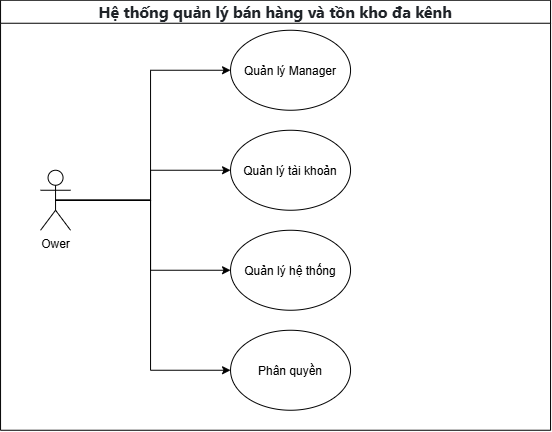
\includegraphics[
        width=0.92\textwidth,
        keepaspectratio
    ]{figures/oner.png}
    \caption{Sơ đồ Use Case của Owner}
    \label{fig:uml-usecase-owner}
\end{figure}


\begin{figure}[H]
    \centering
    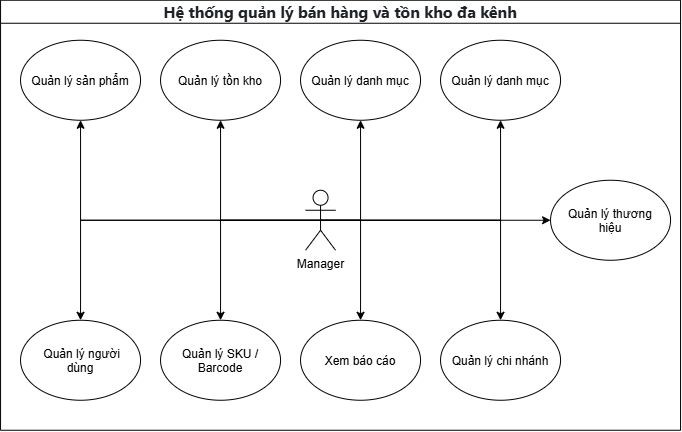
\includegraphics[
        width=0.92\textwidth,
        keepaspectratio
    ]{figures/manager.png}
    \caption{Sơ đồ Use Case của Manager}
    \label{fig:uml-usecase-manager}
\end{figure}

\begin{figure}[H]
    \centering
    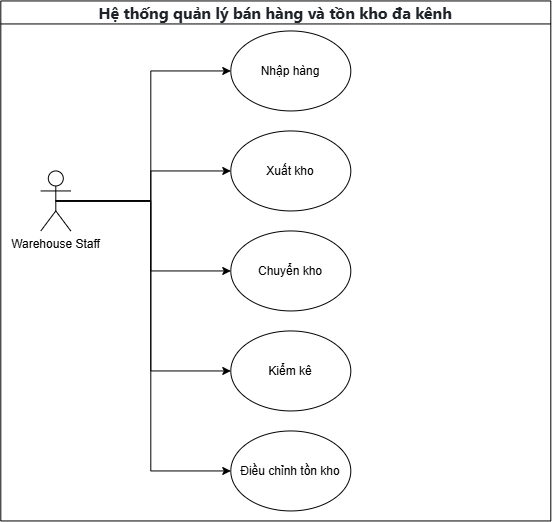
\includegraphics[
        width=0.92\textwidth,
        keepaspectratio
    ]{figures/warehouse.png}
    \caption{Sơ đồ Use Case của Warehouse Staff}
    \label{fig:uml-usecase-warehouse}
\end{figure}

\begin{figure}[H]
    \centering
    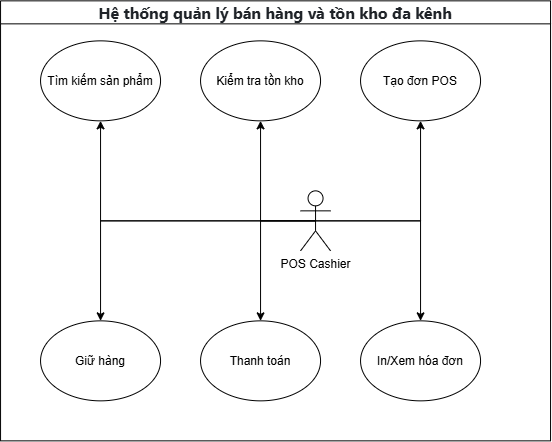
\includegraphics[
        width=0.92\textwidth,
        keepaspectratio
    ]{figures/pos.png}
    \caption{Sơ đồ Use Case của POS}
    \label{fig:uml-usecase-pos}
\end{figure}

\section{Sơ đồ Class}

Sơ đồ Class mô tả các lớp chính và mối quan hệ giữa các lớp trong hệ thống.

\begin{figure}[H]
    \centering
    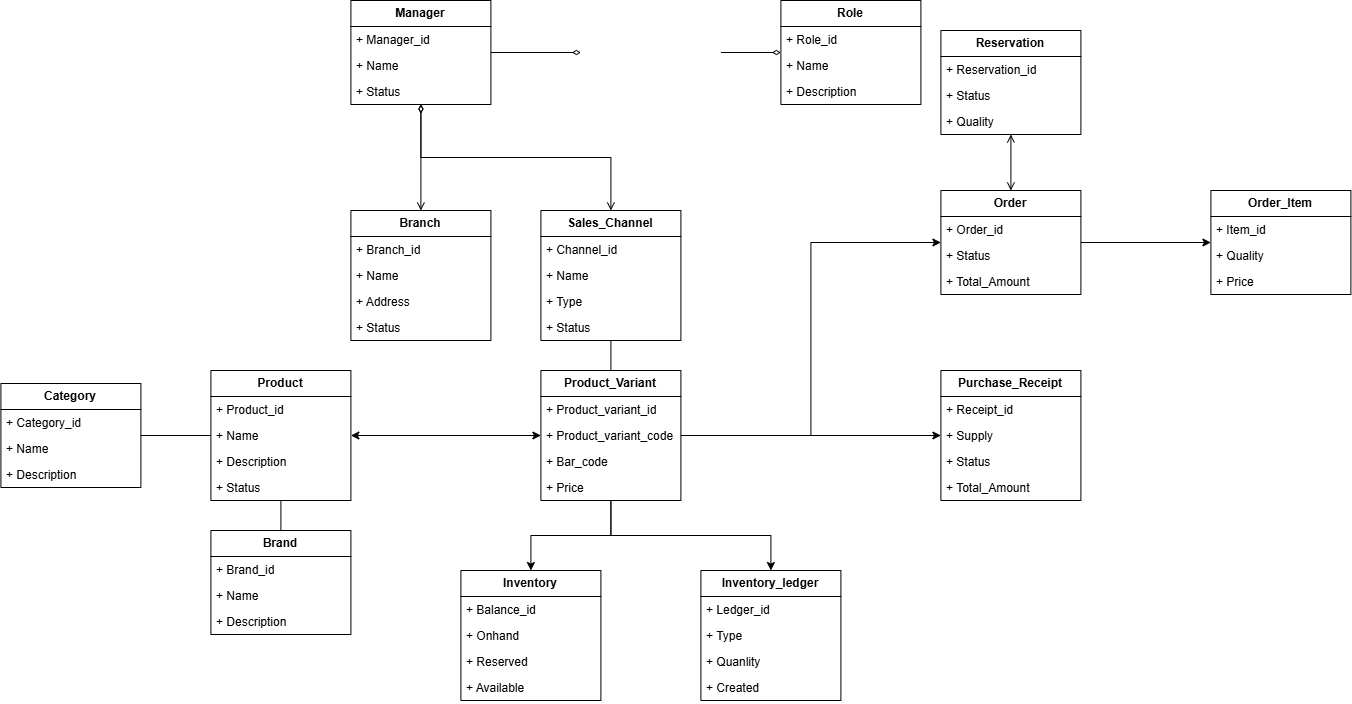
\includegraphics[
        width=0.92\textwidth,
        keepaspectratio
    ]{figures/Class.png}
    \caption{Sơ đồ Class}
    \label{fig:uml-class}
\end{figure}

\section{Sơ đồ Sequence -- Giữ hàng}

Sơ đồ Sequence mô tả trình tự xử lý khi hệ thống thực hiện giữ hàng cho một đơn hàng.

\begin{figure}[H]
    \centering
    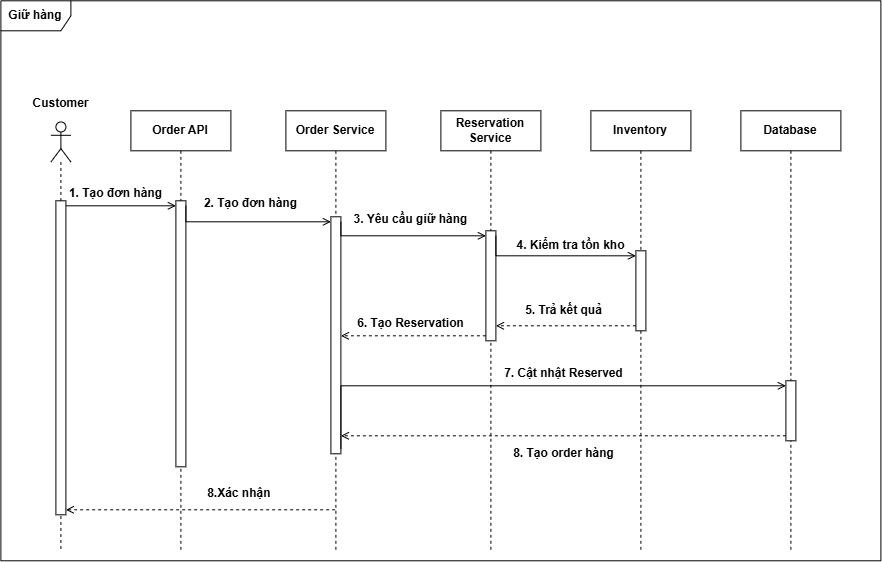
\includegraphics[
        width=0.92\textwidth,
        keepaspectratio
    ]{figures/giữ hàng.png}
    \caption{Sơ đồ Sequence cho nghiệp vụ giữ hàng}
    \label{fig:uml-sequence-reservation}
\end{figure}

\section{Sơ đồ Sequence -- Thanh toán nhanh}

Sơ đồ Sequence mô tả trình tự xử lý của quy trình thanh toán nhanh tại POS.

\begin{figure}[H]
    \centering
    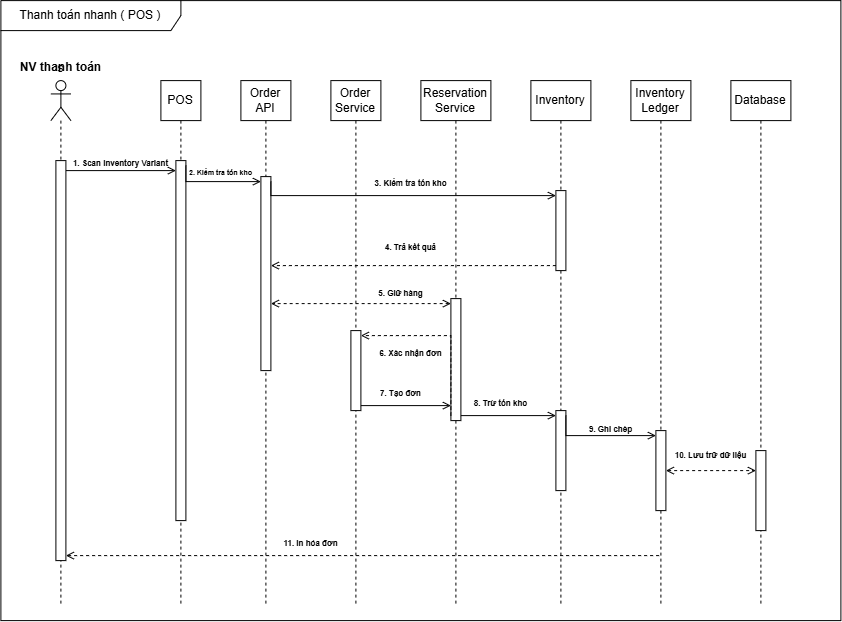
\includegraphics[
        width=0.92\textwidth,
        keepaspectratio
    ]{figures/cash.png}
    \caption{Sơ đồ Sequence cho nghiệp vụ thanh toán nhanh}
    \label{fig:uml-sequence-checkout}
\end{figure}

\section{Sơ đồ Activity}

Sơ đồ Activity mô tả luồng hoạt động chính của một nghiệp vụ tiêu biểu trong hệ thống.

\begin{figure}[H]
    \centering
    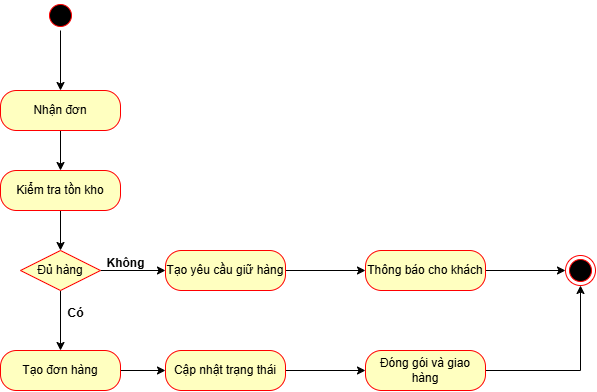
\includegraphics[
        width=0.92\textwidth,
        keepaspectratio
    ]{figures/ad xử lý.png}
    \caption{Sơ đồ Activity cho nghiệp vụ thanh toán nhanh}
    \label{fig:uml-activity-checkout}
\end{figure}

\section{Sơ đồ State}

Sơ đồ State mô tả các trạng thái và quá trình chuyển trạng thái của đơn hàng.
\begin{figure}[H]
    \centering
    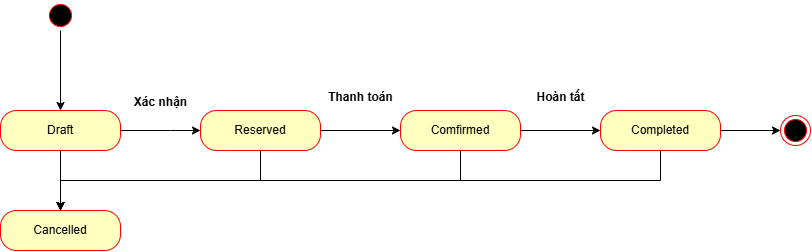
\includegraphics[
        width=0.92\textwidth,
        keepaspectratio
    ]{figures/sd đơn hàng.png}
    \caption{Sơ đồ State cho đơn hàng}
    \label{fig:uml-state}
\end{figure}